% Lambda — A 4 mm² Open-Source Transformer Inference ASIC
% Alan Schwartz, The University of Texas at Austin
% Longhorn Silicon Project · https://github.com/LonghornSilicon
%
% Compile: pdflatex lambda && bibtex lambda && pdflatex lambda && pdflatex lambda
% Or upload to Overleaf as-is.

\documentclass[conference]{IEEEtran}

\usepackage[utf8]{inputenc}
\usepackage{cite}
\usepackage{amsmath,amssymb,amsfonts}
\usepackage{graphicx}
\usepackage{textcomp}
\usepackage{xcolor}
\usepackage{booktabs}
\usepackage{tikz}
\usepackage{pgfplots}
\usetikzlibrary{shapes,arrows.meta,positioning,calc,fit,backgrounds,patterns}
\pgfplotsset{compat=1.18}
\usepackage{url}
\usepackage{microtype}
\usepackage{hyperref}
\hypersetup{
    colorlinks=true,
    linkcolor=black,
    citecolor=blue!60!black,
    urlcolor=blue!60!black,
}

% Compact spacing — keep the paper from bloating
\setlength{\textfloatsep}{8pt plus 2pt minus 2pt}
\setlength{\floatsep}{8pt plus 2pt minus 2pt}
\setlength{\intextsep}{8pt plus 2pt minus 2pt}

% --- Custom abstract: render "Abstract" as a proper centered bold header
%     instead of IEEEtran's inline "Abstract---" prefix.
\renewenvironment{abstract}
  {\par\vspace{4pt}\noindent\begin{center}\textbf{\large Abstract}\end{center}\vspace{-2pt}\par\itshape\small}
  {\par\vspace{6pt}\upshape\normalsize}

\def\BibTeX{{\rm B\kern-.05em{\sc i\kern-.025em b}\kern-.08em
    T\kern-.1667em\lower.7ex\hbox{E}\kern-.125emX}}

\begin{document}

\title{Lambda: A 4\,mm$^2$ Open-Source Transformer Inference ASIC \\ with Streaming Per-Channel KV Compression and Adaptive-Precision KV}

\author{
\IEEEauthorblockN{Alan Schwartz}
\IEEEauthorblockA{Longhorn Silicon Project \\
The University of Texas at Austin \\
\texttt{aschwartz0408@utexas.edu} \\
\url{https://github.com/LonghornSilicon}}
}

\maketitle

\begin{abstract}
\boldmath
We present \textbf{Lambda}, a 4\,mm$^2$ standalone transformer-decode ASIC at TSMC N16FFC, designed for tape-out via the IMEC / Europractice mini@sic 2.0 academic shuttle program. Lambda runs W4A8 transformer models up to 1.5\,B parameters---validated on Qwen2-1.5B---at 6--8\,tokens/s decode in a 2.6\,W typical envelope, on a single LPDDR5X-8533 x16 channel sustaining 12\,GB/s. Three architectural contributions distinguish the chip. \textbf{(1)} We implement \emph{ChannelQuant}, a streaming per-channel KV-compression codec, in silicon: per-channel INT4 keys (grouped, $G{=}128$, with per-channel FP16 scales), per-token INT4 values, and a static top-$k$ ($k{=}2$) FP16 outlier-channel lane selected by a calibrated ROM mask. The recipe follows KIVI~\cite{kivi} and KVQuant~\cite{kvquant}; our contribution is the streaming silicon implementation. Measured compression is $\approx$3.8$\times$ versus FP16 at $\approx$4 bits per value, near-lossless (HellaSwag acc\_norm within $\approx$0.4--0.8\,pt of FP16 at the CQ-4+ tier on Qwen2-0.5B/1.5B). \textbf{(2)} A single shared FP16 compute unit (scale / quantize / dequantize) is serialized across the head-dimension channels---a single divide cone---and keys are dequantized per-channel (INT4$\,\cdot\,$FP16) \emph{before} the score matmul; there is no compressed-domain read path. \textbf{(3)} We introduce a Token Importance Unit (TIU): a 0.03\,mm$^2$ block that accumulates per-block attention entropy and drives both heavy-hitter eviction and adaptive per-block ChannelQuant-tier selection in the KV cache. The complete chip integrates seven functional units under an ACU/MSC/LSU/TIU/HIF top-level hierarchy and presents a PCIe Gen3 x1 host interface on an M.2 2280 form factor. We document the design-space exploration that led to the 4\,mm$^2$ target, the LPDDR5X-vs-LPDDR4X PHY tradeoff that gates the model-class commitment, and an explicit pre-RTL audit of the spec. Physical PPA numbers for the KV-compression block at N16FFC (area, power, $F_\mathrm{max}$) are pending re-measurement for ChannelQuant. Lambda is, to our knowledge, the first open-source academic standalone transformer accelerator targeting the small-model ($\leq$1.5\,B-parameter) on-device deployment regime.
\unboldmath
\end{abstract}

\begin{IEEEkeywords}
LLM inference accelerator, KV-cache compression, ChannelQuant, per-channel quantization, FlashAttention, paged attention, adaptive precision, TSMC N16FFC, academic ASIC, IMEC mini@sic
\end{IEEEkeywords}

% =====================================================================
\section{Introduction}
% =====================================================================

The small-model transformer---up to a few billion parameters---has become the practical on-device deployment regime for large language models in 2025--2026. Qwen2-1.5B~\cite{qwen25}, Llama-3.2-1B/3B~\cite{llama3}, Mistral-NeMo~\cite{mistral_nemo}, Phi-3.5-mini~\cite{phi35}, and Gemma-2-2B all target this band; Apple's recently-published foundation-language-model family~\cite{apple_foundation}, Google Gemini Nano, and Microsoft Copilot+ all deploy at similar scales. The accelerators that serve these workloads in production---Apple's Neural Engine, Qualcomm's Hexagon NPU---are proprietary integrated SoCs whose internal architectures are not publicly documented. Modern GPU accelerators~\cite{nvidia_ampere,nvidia_hopper,nvidia_blackwell} serve the workload at the data-center scale but at die areas and power envelopes 10$^2$--10$^3$ times Lambda's. No open-source academic standalone accelerator at this model class and process node currently exists.

Lambda fills that gap. We present a 4\,mm$^2$ ASIC at TSMC N16FFC, designed for tape-out through the IMEC / Europractice mini@sic 2.0 academic shuttle program~\cite{imec_minisic} at a shuttle cost of approximately \$60--100\,K. The chip runs a W4A8 transformer up to 1.5\,B parameters (validated on Qwen2-1.5B) at 6--8 decode tokens per second in a 2.6\,W typical envelope, holding 4--8\,GB of weights in an off-chip LPDDR5X-8533 x16 package and exposing host I/O over a PCIe Gen3 x1 link on an M.2 2280 carrier card.

Three architectural commitments differentiate Lambda from prior open-source accelerator designs:

\textbf{(1) Streaming per-channel KV compression in silicon (ChannelQuant).} Lambda's KV-compression engine (KVE) implements \emph{ChannelQuant}: per-channel INT4 keys (grouped, $G{=}128$, with per-channel FP16 scales), per-token INT4 values (INT8 in the CQ-8 tier), and a static top-$k$ ($k{=}2$) FP16 outlier-channel lane selected by a calibrated ROM mask. Keys and values share a single per-channel SRAM record and one serialized FP16 scale/quantize/dequantize unit. The recipe follows KIVI~\cite{kivi} and KVQuant~\cite{kvquant}; our contribution is the streaming silicon implementation. Measured compression is $\approx$3.8$\times$ versus FP16 at $\approx$4 bits per value (4.13--4.38 depending on head dimension $D$), near-lossless: HellaSwag acc\_norm falls within $\approx$0.4--0.8\,pt of FP16 at the CQ-4+ tier on Qwen2-0.5B/1.5B. The full block RTL is complete through Sky130 sign-off; physical PPA at N16FFC is pending re-measurement.

\textbf{(2) Per-channel dequantization before scoring.} The datapath serializes one shared FP16 compute unit across the $D$ head-dimension channels (a single divide cone), and keys are reconstructed per-channel (INT4\,$\cdot$\,FP16, with FP16 replay for the $k{=}2$ outlier channels) \emph{before} the attention dot product. Lambda's matrix engine (MatE) therefore keeps weight and FFN GEMMs at INT8\,$\times$\,INT4 and scores Q\,$\cdot$\,K$^\top$ on the dequantized K (INT8 Q $\times$ dequantized FP16 K); there is no compressed-domain / raw-index read path, and the KV codec itself needs no fallback to FP16. FP16 multiplication in MatE is confined to the per-tile P\,$\cdot$\,V escape (\S\ref{sec:dataflow}, selected by the ACU precision controller); the remaining FP16 work is in VecU (softmax, RMSNorm, RoPE, SiLU) and the KVE's shared scale unit.

\textbf{(3) Token Importance Unit (TIU) for adaptive precision.} Inspired by the entropy-driven KV quantization analysis of~\cite{adaptive_kv}, we introduce a small (0.03\,mm$^2$) on-die accumulator that tracks the cumulative softmax weight per 16-token KV block. The TIU output drives two consumer paths: a heavy-hitter eviction policy in the memory subsystem controller (H2O-style retention~\cite{h2o}) and a per-block ChannelQuant-tier selector that keeps high-importance blocks at a higher tier (CQ-4+ or CQ-8) and demotes low-importance blocks to CQ-4. To our knowledge, this is the first silicon implementation of adaptive-precision KV cache management; published prior work is software-only.

The remainder of this paper develops these contributions in detail. Section~\ref{sec:background} surveys the prior art the design is grounded in. Section~\ref{sec:architecture} describes Lambda's seven functional blocks and their top-level grouping. Section~\ref{sec:dataflow} traces the decode token data flow and the quantization decisions that shape it. Section~\ref{sec:implementation} reports the area and power budgets, including a pre-RTL audit that corrected eight numerical inconsistencies in the original spec. Section~\ref{sec:performance} characterizes Lambda's coverage across the candidate-model space and quantifies the load-bearing LPDDR5X-vs-LPDDR4X PHY tradeoff. Section~\ref{sec:discussion} discusses what we deliberately excluded and why.

% =====================================================================
\section{Background and Related Work}
\label{sec:background}
% =====================================================================

Lambda integrates four lines of recent research into a single chip target.

\textbf{Online attention.} The running-max/running-sum softmax recurrence originates with~\cite{onlinesoftmax}; FlashAttention~\cite{flashattention,flashattention2,flashattention3} wraps that same recurrence in an IO-aware tiled reduction (per-row running maxima $m_i$ and running sums-of-exponentials $\ell_i$), eliminating materialization of the score matrix and reducing the activation-memory pressure that dominates long-context attention. Lambda's vector unit (VecU) implements this online-softmax recurrence in microcode --- the algorithm is identical across FlashAttention-1/2/3, and FA-3's distinctive Hopper-specific asynchrony and FP8 paths are \emph{not} used here; the running state per row is two FP16 scalars plus the running output accumulator $O_i$. VecU also implements the rotary positional embedding scheme (RoPE)~\cite{rope}, RMSNorm~\cite{rmsnorm}, and the SwiGLU gating used by the Llama-3 family~\cite{swiglu} as microcoded loops.

\textbf{Paged KV management.} vLLM's PagedAttention~\cite{pagedattention} treats the KV cache as a virtual address space with fixed-size physical blocks, indexed by a per-sequence block table. The pattern enables zero-fragmentation memory use and dynamic eviction. Lambda's memory subsystem controller (MSC) implements this in silicon as a 128-entry content-addressable block table with 16-token blocks, the silicon analog of vLLM's logical-to-physical mapping. FlashInfer~\cite{flashinfer} extends the paged abstraction to a composable taxonomy of attention patterns (dense paged, sparse structured, ragged, composite); Lambda's MSC exposes a CSR-selectable mode covering this taxonomy.

\textbf{Weight and activation quantization.} W4A8 has emerged as the production sweet spot for small-LLM inference~\cite{w4a8_acl25}: 4-bit weights (via GPTQ~\cite{gptq} or AWQ~\cite{awq}) and 8-bit per-token dynamic activations (via SmoothQuant~\cite{smoothquant}) preserve quality on the small-model class within a few MMLU points of FP16. Lambda's MatE multiplies INT8 activations against INT4 weights as its primary path.

\textbf{KV-cache compression.} A growing body of work~\cite{kivi,kvquant,kv_survey,quarot,rotatekv,turboquant} compresses KV caches via uniform quantization, per-channel/per-token quantization, rotation, codebook quantization, or per-token mixed precision. KIVI~\cite{kivi} establishes the asymmetric recipe Lambda adopts---\emph{per-channel} quantization for keys (each channel gets its own scale, so a large-magnitude channel does not coarsen the whole tile) and \emph{per-token} quantization for values---and KVQuant~\cite{kvquant} adds a dense-and-sparse split that keeps a small set of outlier channels in high precision. Lambda's ChannelQuant codec follows this recipe: per-channel INT4 keys (grouped $G{=}128$), per-token INT4 values, and a static top-$k$ ($k{=}2$) FP16 outlier-channel lane. Rotation-codebook methods such as TurboQuant~\cite{turboquant} are a different point in the design space (Walsh--Hadamard rotation plus a Lloyd--Max scalar codebook); we cite them as prior work but do not implement them. Because keys are dequantized per-channel (INT4\,$\cdot$\,FP16) before scoring, Lambda's codec needs no compressed-domain read trick, and Q\,$\cdot$\,K$^\top$ scores on dequantized K with no fallback to FP16 in the KV read path. FP16 in MatE is confined to the per-tile P\,$\cdot$\,V escape (\S\ref{sec:dataflow}): the P\,$\cdot$\,V matmul does adopt a per-tile INT8/FP16 route in the manner of adaptive-precision designs~\cite{adaptive_kv,chaithu_acu}, while weight/FFN GEMMs stay INT8\,$\times$\,INT4.

\textbf{Attention-weight-driven eviction and adaptive precision.} H2O~\cite{h2o}, Scissorhands~\cite{scissorhands}, TOVA~\cite{tova}, and the StreamingLLM ``attention-sink'' phenomenon~\cite{streamingllm} all show that retaining tokens whose cumulative attention weight exceeds a threshold (and evicting the rest) preserves long-context quality at a fraction of the KV-cache footprint. The recent adaptive-precision-KV work~\cite{adaptive_kv} extends this idea to bit-width allocation: high-attention tokens stay at higher precision, low-attention tokens demote. Lambda's TIU is the silicon expression of this idea at per-block granularity (16 tokens per block, matching the PagedAttention block size).

% =====================================================================
\section{Architecture}
\label{sec:architecture}
% =====================================================================

Figure~\ref{fig:topology} shows Lambda's top-level decomposition. Seven functional blocks are grouped under five top-level units---ACU (Attention Compute Unit), MSC (Memory Subsystem Controller), LSU (Layer Sequencer), TIU (Token Importance Unit), and HIF (Host Interface)---plus 0.8\,MB of on-die SRAM in four banks and a vendor-IP LPDDR5X x16 PHY. The ACU is itself a composite of three blocks (MatE, VecU, KVE) that share the compute fabric of the chip; the naming convention follows~\cite{chaithu_acu} while preserving the internal block structure for high-level synthesis (HLS) modularity. We discuss each block in turn.

% --- Figure 1: top-level architecture (full page width) ---
\begin{figure*}[t]
\centering
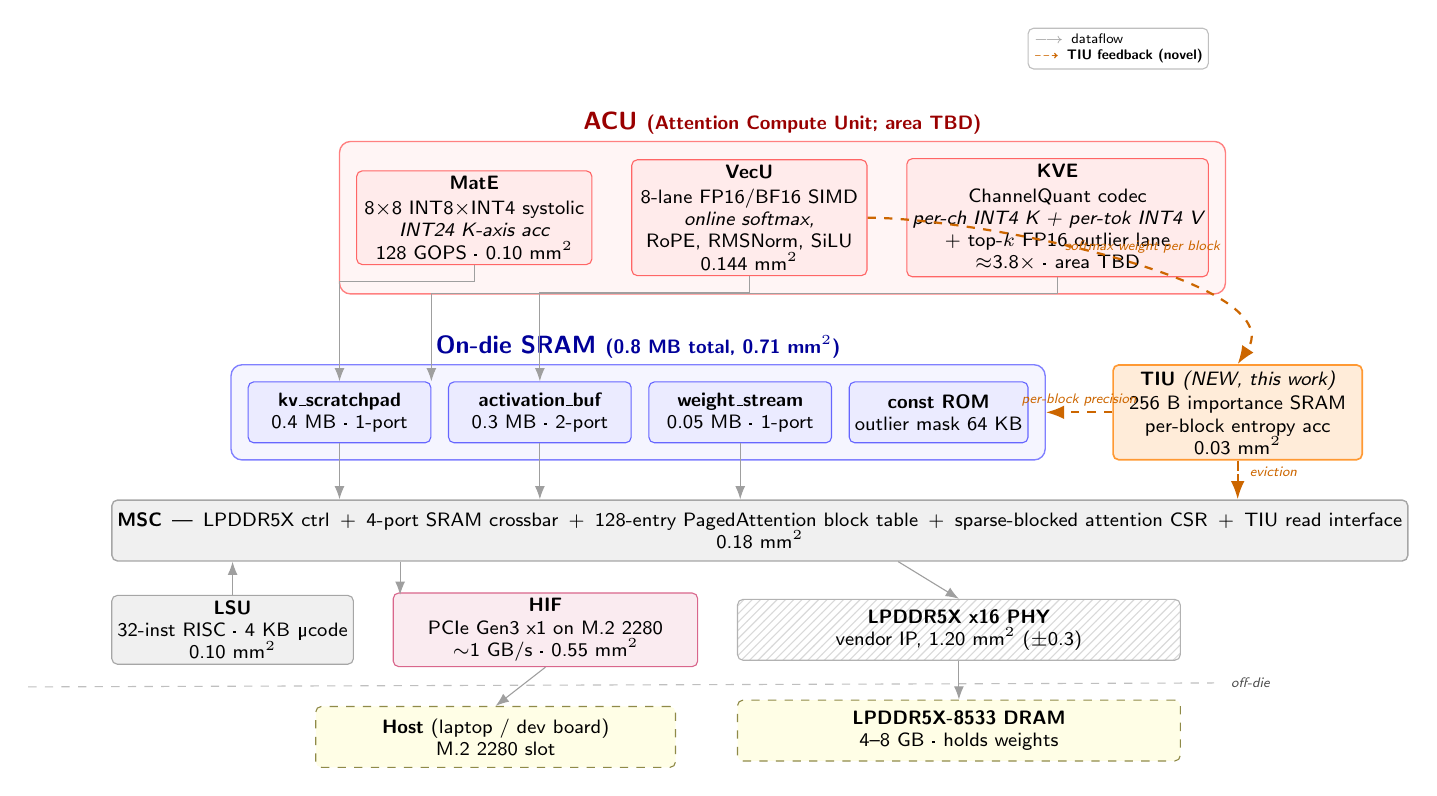
\begin{tikzpicture}[
  font=\sffamily\footnotesize,
  every node/.style={inner sep=2pt},
  block/.style={draw, rounded corners=2pt, minimum height=22pt, align=center, font=\sffamily\scriptsize},
  acu/.style={block, fill=red!8, draw=red!60, line width=0.4pt},
  mem/.style={block, fill=blue!8, draw=blue!60, line width=0.4pt},
  msc/.style={block, fill=gray!12, draw=gray!70, line width=0.5pt},
  lsu/.style={block, fill=gray!12, draw=gray!70, line width=0.4pt},
  tiunode/.style={block, fill=orange!15, draw=orange!80, line width=0.6pt},
  hif/.style={block, fill=purple!8, draw=purple!60, line width=0.4pt},
  phy/.style={block, fill=gray!5, draw=gray!60, line width=0.4pt, pattern=north east lines, pattern color=gray!30},
  offdie/.style={block, fill=yellow!10, draw=yellow!50!black, dashed, line width=0.4pt},
  arrow/.style={-Latex, thin, gray!75},
  fbarrow/.style={-Latex, thick, orange!80!black, dashed},
  group/.style={draw, rounded corners=4pt, line width=0.5pt, inner sep=6pt},
  acugroup/.style={group, draw=red!50, fill=red!4},
  memgroup/.style={group, draw=blue!50, fill=blue!4},
]

% =============================================================
% Top tier: ACU (compute fabric)
% =============================================================
\node[acu, minimum width=85pt] (mate) at (0,4.2)
  {{\bfseries MatE}\\[1pt]\scriptsize 8$\times$8 INT8$\times$INT4 systolic\\\scriptsize \itshape INT24 K-axis acc\\\scriptsize 128 GOPS · 0.10 mm$^2$};
\node[acu, minimum width=85pt, right=14pt of mate] (vecu)
  {{\bfseries VecU}\\[1pt]\scriptsize 8-lane FP16/BF16 SIMD\\\scriptsize \itshape online softmax,\\\scriptsize RoPE, RMSNorm, SiLU\\\scriptsize 0.144 mm$^2$};
\node[acu, minimum width=85pt, right=14pt of vecu] (kce)
  {{\bfseries KVE}\\[1pt]\scriptsize ChannelQuant codec\\\scriptsize \itshape per-ch INT4 K + per-tok INT4 V\\\scriptsize + top-$k$ FP16 outlier lane\\\scriptsize $\approx$3.8$\times$ · area TBD};
\begin{scope}[on background layer]
\node[acugroup, fit=(mate)(vecu)(kce),
      label={[red!60!black, font=\sffamily\small\bfseries, anchor=south]above:ACU \scriptsize (Attention Compute Unit; area TBD)}] (acu) {};
\end{scope}

% =============================================================
% Middle tier: SRAM banks (left) + TIU (right, novel)
% =============================================================
\node[mem, minimum width=66pt, below=42pt of mate.south west, xshift=-6pt] (kvs)
  {{\bfseries kv\_scratchpad}\\\scriptsize 0.4 MB · 1-port};
\node[mem, minimum width=66pt, right=6pt of kvs] (actb)
  {{\bfseries activation\_buf}\\\scriptsize 0.3 MB · 2-port};
\node[mem, minimum width=66pt, right=6pt of actb] (wsb)
  {{\bfseries weight\_stream}\\\scriptsize 0.05 MB · 1-port};
\node[mem, minimum width=44pt, right=6pt of wsb] (rom)
  {{\bfseries const ROM}\\\scriptsize outlier mask 64 KB};

\begin{scope}[on background layer]
\node[memgroup, fit=(kvs)(actb)(wsb)(rom),
      label={[blue!60!black, font=\sffamily\small\bfseries, anchor=south]above:On-die SRAM \scriptsize (0.8 MB total, 0.71 mm$^2$)}] (sram) {};
\end{scope}

% TIU --- novel block, highlighted
\node[tiunode, minimum width=90pt, right=24pt of sram] (tiu)
  {{\bfseries TIU} {\scriptsize\itshape (NEW, this work)}\\[1pt]\scriptsize 256 B importance SRAM\\\scriptsize per-block entropy acc\\\scriptsize 0.03 mm$^2$};

% =============================================================
% MSC (full-width bar)
% =============================================================
\node[msc, minimum width=420pt, below=14pt of sram.south, anchor=north, xshift=44pt] (msc)
  {{\bfseries MSC} \,---\, LPDDR5X ctrl \,+\, 4-port SRAM crossbar \,+\, 128-entry PagedAttention block table \,+\, sparse-blocked attention CSR \,+\, TIU read interface\\
   \scriptsize 0.18 mm$^2$};

% =============================================================
% Bottom-left: LSU + HIF
% =============================================================
\node[lsu, minimum width=85pt, below=12pt of msc.south west, anchor=north west] (lsu)
  {{\bfseries LSU}\\\scriptsize 32-inst RISC · 4 KB \textmu code\\\scriptsize 0.10 mm$^2$};

\node[hif, minimum width=110pt, right=14pt of lsu] (hif)
  {{\bfseries HIF}\\\scriptsize PCIe Gen3 x1 on M.2 2280\\\scriptsize $\sim$1 GB/s · 0.55 mm$^2$};

\node[phy, minimum width=160pt, right=14pt of hif] (lpddrphy)
  {{\bfseries LPDDR5X x16 PHY}\\\scriptsize vendor IP, 1.20 mm$^2$ ($\pm$0.3)};

% =============================================================
% Off-die row
% =============================================================
\node[offdie, minimum width=130pt, below=14pt of hif.south, xshift=-18pt] (hostpc)
  {{\bfseries Host} (laptop / dev board)\\\scriptsize M.2 2280 slot};
\node[offdie, minimum width=160pt, below=14pt of lpddrphy.south] (dram)
  {{\bfseries LPDDR5X-8533 DRAM}\\\scriptsize 4--8 GB · holds weights};

% Dashed separator: on-die / off-die
\draw[dashed, gray!50, thin] ($(lsu.south west) + (-30pt,-8pt)$) -- ($(lpddrphy.south east) + (12pt,-8pt)$)
   node[font=\sffamily\tiny, gray!60!black, anchor=west, xshift=4pt] {\itshape off-die};

% =============================================================
% Arrows --- main dataflow (gray, thin)
% =============================================================
\draw[arrow] (mate.south) -- ++(0,-6pt) -| (kvs.north);
\draw[arrow] (vecu.south) -- ++(0,-6pt) -| (actb.north);
\draw[arrow] (kce.south) -- ++(0,-6pt) -| (kvs.north east);
\draw[arrow] (kvs.south) -- ($(msc.north -| kvs.south) + (0,0)$);
\draw[arrow] (actb.south) -- ($(msc.north -| actb.south) + (0,0)$);
\draw[arrow] (wsb.south) -- ($(msc.north -| wsb.south) + (0,0)$);
\draw[arrow] (msc.south) ++(-130pt,0) -- ++(0,-12pt);
\draw[arrow] (msc.south) ++(50pt,0) -- (lpddrphy.north);
\draw[arrow] (lpddrphy.south) -- (dram.north);
\draw[arrow] (hif.south) -- (hostpc.north);
\draw[arrow] (lsu.north) -- (msc.south -| lsu.north);

% =============================================================
% TIU feedback paths --- HIGHLIGHTED (the novel contribution)
% =============================================================
\draw[fbarrow] (vecu.east) ..controls +(40pt,0) and +(20pt,30pt).. (tiu.north)
  node[font=\sffamily\tiny, orange!80!black, midway, above, xshift=10pt]
       {\itshape softmax weight per block};
\draw[fbarrow] (tiu.west) -- (sram.east)
  node[font=\sffamily\tiny, orange!80!black, midway, above]
       {\itshape per-block precision};
\draw[fbarrow] (tiu.south) ..controls +(0,-28pt) and +(0,28pt).. ($(msc.north -| tiu.south)$)
  node[font=\sffamily\tiny, orange!80!black, near end, right, xshift=2pt]
       {\itshape eviction};

% Legend (lifted above the ACU group so it doesn't overlap KCE text)
\node[draw=gray!50, rounded corners=2pt, fill=white, font=\sffamily\tiny, align=left, anchor=south east] at ($(kce.north east) + (0pt,32pt)$)
  {\textcolor{gray!75}{$\longrightarrow$}~\,dataflow \\
   \textcolor{orange!80!black}{$\dashrightarrow$}~\,\textbf{TIU feedback (novel)}};

\end{tikzpicture}
\caption{Lambda's top-level architecture, drawn full page width to keep the dataflow legible. The chip's seven functional blocks are grouped under five top-level units. The \textbf{ACU (Attention Compute Unit, red)} contains the three compute blocks that share the GEMM and SIMD fabric (MatE, VecU, KVE). The four on-die SRAM banks (blue, 0.8\,MB total) sit between the compute fabric and the memory controller. The \textbf{MSC} manages LPDDR access, the 128-entry PagedAttention block table, sparse-blocked attention CSR modes, and the TIU read interface. The \textbf{LSU} walks a pre-compiled 4\,KB microcode schedule. The \textbf{TIU (orange, novel to this work)} accumulates per-block attention entropy from VecU's softmax broadcasts and drives two feedback paths drawn in dashed orange: per-block ChannelQuant-tier selection to the KVE, and heavy-hitter-driven eviction to MSC. The \textbf{HIF} is a PCIe Gen3 x1 endpoint on an M.2 2280 carrier; the LPDDR5X x16 PHY drives the off-die LPDDR5X package. Areas shown are at the PHY mid-case (1.20\,mm$^2$); the KVE block area is pending re-measurement for ChannelQuant.}
\label{fig:topology}
\end{figure*}

\subsection{Matrix Engine (MatE)}

MatE is an 8$\times$8 weight-stationary systolic array of 64 INT8\,$\times$\,INT4 processing elements (PEs). At 1\,GHz, peak throughput is 128\,GOPS; sustained throughput at 60\,\% utilization is 76.8\,GOPS---a figure that is, in the bandwidth-bound regime, 1.6$\times$ the throughput the chip needs at the largest model size. The factor is constant across model sizes in this regime because the GOPS demand scales with bandwidth (not with model size); we found and corrected an earlier draft claim of ``3--5$\times$ headroom'' as a derivation error during the spec audit.

Two dataflow modes are CSR-selectable:

\textit{Weight-stationary} for the GEMMs that dominate transformer compute: Q/K/V projections, attention output projection, FFN up- and down-projections, and the final logits projection. Weights pin once per tile; activations stream from the activation buffer; products accumulate down the columns.

\textit{Output-stationary} for the Q\,$\cdot$\,K$^\top$ attention scoring step. Q vectors pin for the duration of the attention tile; K values stream from the kv\_scratchpad. K is stored in ChannelQuant form (per-channel INT4 codes plus per-channel FP16 scales); the KVE reconstructs it per-channel (INT4\,$\cdot$\,FP16, with FP16 replay for the $k{=}2$ outlier channels) \emph{before} it enters the array, so MatE scores against dequantized K---there is no compressed-domain / raw-index read path. The products feed an INT24 reduction along the head-dimension axis. We selected INT24 (rather than the INT16 the original spec contained) after analysis showed the INT16 width saturates on the FFN reductions of the earlier target-model dims; the INT16 width survives only as the partial-product register inside each PE, following the per-PE/per-column accumulator split of Jouppi's TPU~\cite{jouppi_tpu,tpu_v4}. The exact accumulator margin for the Qwen2-1.5B target is pending re-derivation.

\subsection{Vector Unit (VecU)}

VecU is eight FP16/BF16 SIMD lanes sharing a 1\,K-instruction microcode RAM and three 64-entry transcendental LUTs (\texttt{exp}, \texttt{rsqrt}, \texttt{sigmoid}) with linear interpolation. The unit handles every non-GEMM operation in the transformer: the online-softmax recurrence, rotary positional embedding (RoPE) pair-rotation, RMSNorm, SiLU/GELU, residual addition, and sampling. We chose programmable SIMD over fixed-function blocks for verification economy---one microcoded block has a smaller verification surface than four fixed-function blocks.

The online softmax microcode is the most consequential program. Per attention row, VecU maintains a triple $(m_i, \ell_i, O_i)$: running max, running sum-of-exponentials, and running output accumulator. As each tile of scores arrives, VecU computes the new max, rescales the running accumulators by $e^{m_{\mathrm{old}} - m_{\mathrm{new}}}$, exponentiates the tile via the exp LUT, and accumulates into $\ell_i$ and into $O_i$ weighted by the corresponding V tile. The 8 lanes parallelize across rows; tile size is 32--64 scores; approximately 32 microinstructions execute per tile.

\subsection{KV Cache Engine (KVE) --- ChannelQuant}

The KVE is the headline research IP: a streaming silicon implementation of \emph{ChannelQuant}. It compresses keys and values as MatE produces them and reconstructs them per-channel on the read path. For keys, the KVE buffers a group of $G{=}128$ keys, takes the per-channel absolute maximum over the group, derives $D$ per-channel FP16 scales, and quantizes each channel to INT4; the static top-$k$ ($k{=}2$) outlier channels---selected by a calibrated ROM mask---bypass INT4 and are held in FP16. Values are quantized per token to INT4 (INT8 in the CQ-8 tier). Keys and values live in a unified per-channel SRAM record $\{\text{tag},\ D{\times}\text{FP16 scale},\ D{\times}\text{INT4 code}\}$. Decompression is per-channel $\text{INT4}\cdot\text{FP16}$, with FP16 replay for the outlier channels. Measured cost is $\approx$4 bits per value (4.13--4.38 depending on head dimension $D$), i.e.\ $\approx$3.8$\times$ versus FP16, and near-lossless (HellaSwag acc\_norm within $\approx$0.4--0.8\,pt of FP16 at CQ-4+ on Qwen2-0.5B/1.5B). The recipe follows KIVI~\cite{kivi} and KVQuant~\cite{kvquant}; our contribution is the streaming silicon datapath.

The datapath serializes a \emph{single} shared FP16 compute unit (scale, quantize, dequantize) across the $D$ head-dimension channels---one divide cone reused on both the compress and decompress paths---rather than a wide parallel array. Three tiers plus a bypass are CSR-selectable: \textbf{CQ-8} (per-token INT8 K and V), \textbf{CQ-4} (per-channel INT4 K, per-token INT4 V; the primary tier), \textbf{CQ-4+} (CQ-4 plus the $k{=}2$ FP16 outlier channels; the near-lossless tier), and an FP16 bypass for ablation. The full block RTL is complete through Sky130 sign-off in the \texttt{kv-cache-engine} repository; the physical PPA of the block at N16FFC (area, power, $F_\mathrm{max}$) is pending re-measurement for ChannelQuant.

\subsection{Memory Subsystem Controller (MSC)}

MSC integrates four functions in 0.18\,mm$^2$: the LPDDR5X x16 protocol-side controller (with open-page policy and bank-conflict avoidance), a 4-port SRAM crossbar serving MatE, VecU, KVE, and the host, a 128-entry block table providing the silicon analog of vLLM's PagedAttention~\cite{pagedattention} indexing (16 tokens per block, 2\,K addressable tokens per session), and a DMA descriptor FSM. Sparse-blocked attention is exposed as a CSR-selectable mode (\texttt{attention\_pattern\_modes}) following the FlashInfer taxonomy~\cite{flashinfer}: dense paged, sliding window, sparse blocked, local+global hybrid (the Gemma-2 layout).

MSC is single-session by design. We exclude continuous batching (multi-session state), tier-3 host-DRAM eviction (we have no PCIe-to-host swap path on a 4\,mm$^2$ die), and cross-session prefix sharing. These omissions are deliberate: the chip is sized for batch-1 on-device inference, not multi-tenant serving.

\subsection{Layer Sequencer (LSU)}

The LSU is a minimal three-stage in-order RISC: 32-bit fixed-width instruction format, 32 instructions, 16 $\times$ 32-bit general-purpose registers, 4\,KB of microcode RAM holding the entire pre-compiled per-layer schedule, single-issue across three dispatch lanes (scalar, vector to ACU, DMA to MSC). No branch predictor, no out-of-order machinery, no cache hierarchy: transformer decode is structurally identical layer to layer, and a static schedule walked deterministically suffices. The host loads roughly 3\,K microcode instructions at boot; the chip executes the same schedule forever. The footprint is 0.10\,mm$^2$.

\subsection{Token Importance Unit (TIU)}

TIU is a 0.03\,mm$^2$ block introduced in this work. It maintains a 256-byte importance SRAM organized as 128 entries of 16 bits each (one entry per PagedAttention block). Update path: VecU broadcasts the per-block cumulative softmax weight of the current attention pass; the TIU adds to the corresponding importance register. Consumer paths: (i) MSC queries the lowest-importance block when the kv\_scratchpad approaches capacity (heavy-hitter eviction, H2O-style~\cite{h2o}), and (ii) the KVE queries the per-block importance bucket when re-compressing an evicted-and-recalled block, demoting low-importance blocks to the CQ-4 tier while keeping high-importance blocks at a higher tier (CQ-4+ or CQ-8).

Four CSR-selectable policies cover the design space: \texttt{tiu\_off} (pure FIFO eviction, uniform precision), \texttt{tiu\_h2o} (heavy-hitter retention, uniform precision), \texttt{tiu\_streaming\_llm} (recent + attention-sink retention), and \texttt{tiu\_adaptive\_precision} (heavy-hitter retention plus per-block adaptive precision). The block is grounded in the adaptive-precision-KV analysis of~\cite{adaptive_kv}, which we believe has not previously been implemented in silicon.

\subsection{Host Interface (HIF)}

HIF is a PCIe Gen3 x1 endpoint (~1\,GB/s sustained) on the M.2 2280 form factor at the PCB level. The M.2 connector wires four PCIe lanes by specification; Lambda drives only one on-die, and PCIe link training negotiates the link down to x1. Vendor IP (Synopsys DesignWare or Cadence's PCIe Gen3 PHY at 16\,nm) provides the analog and protocol stack; we implement the BAR0 CSR map, the 16-deep doorbell command queue, and the JTAG TAP. JTAG runs on dedicated pins, separate from the PCIe lanes, so post-silicon debug remains accessible before PCIe link is up. Total block area is 0.55\,mm$^2$, of which the vendor PHY accounts for approximately 0.35\,mm$^2$.

We initially specified USB-C 2.0 for this interface and revised to PCIe Gen3 x1 mid-design after concluding that the 25-second weight-load latency of USB-C 2.0 was a development-iteration cost we did not want to accept, and that the M.2 form factor better matched the modern inference-card target. The PCIe vendor IP also has public 16\,nm datasheets, in contrast to the LPDDR5X x16 PHY which remains NDA-gated at 16\,nm; the PCIe-side risk profile is therefore lower.

% =====================================================================
\section{Dataflow and Quantization}
\label{sec:dataflow}
% =====================================================================

We walk one decode token through the pipeline to make the quantization commitments concrete. For continuity with the earlier design iterations we use a 3-billion-parameter model as the illustrative example (Llama-3.2-3B, 28 layers, 8 KV heads of 128 dimensions, 3072 hidden width, FFN width 8192); the canonical target is smaller (Qwen2-1.5B), and the per-layer/per-token \emph{timing} figures in this example are pending re-derivation for that target.

The LSU issues approximately 200 microinstructions per layer. For each layer, the schedule alternates four operand-stationary patterns. \textbf{(1) Q/K/V projection:} MatE consumes the activation vector and three weight matrices (streamed from LPDDR via the weight\_stream\_buffer), in weight-stationary mode, producing three 1024-dimensional output vectors. \textbf{(2) RoPE rotation:} VecU rotates Q and K pair-wise using the rotary frequency table. \textbf{(3) KV compression:} the KVE compresses the new K per-channel (INT4 codes plus $D$ FP16 scales, $k{=}2$ outlier channels held FP16) and the new V per-token (INT4), writing the unified per-channel record into the kv\_scratchpad. \textbf{(4) Attention scoring:} MatE switches to output-stationary mode and computes Q\,$\cdot$\,K$^\top$ against K that the KVE has \textit{dequantized per-channel} (INT4\,$\cdot$\,FP16) just ahead of the array. The multiplier path is INT8 (Q) $\times$ dequantized K, and the K-axis reduction is INT24. There is no compressed-domain / raw-index read path.

The scores feed VecU, which executes the online-softmax microcode in tiles of 32. Simultaneously, the running output accumulator $O_i$ is updated by multiplying scaled scores against the V values (dequantized per-token by the KVE) through the same MatE path; this P\,$\cdot$\,V matmul is the one place MatE routes precision per tile (INT8 or FP16, \S\ref{sec:pv-precision}). When the last tile is consumed, $O_i$ is the attention output. The TIU has been quietly accumulating the per-block cumulative softmax weight throughout this loop; the importance SRAM is now ready for the next eviction or precision-tuning decision.

The post-attention path runs through MatE again (attention output projection, FFN up-projection, FFN down-projection) and VecU (SiLU, residual add, RMSNorm). Compute is bandwidth-bound throughout: the limiting factor is the time required to stream the weights of each linear layer from LPDDR5X, giving a 6--8 tokens-per-second decode cadence for the target model class. (The per-layer and per-token timing figures were derived for the retired 3--5\,B example set and are pending re-derivation for the Qwen2-1.5B target.)

\subsection{Adaptive precision: the FP16 P\,$\cdot$\,V path}
\label{sec:pv-precision}

Adaptive-precision-attention designs~\cite{adaptive_kv,chaithu_acu} route ``outlier'' attention tiles to an FP16 multiplier and ``inlier'' tiles to an INT8 multiplier, with a per-tile gating function deciding which path to take. The rationale is that some attention tiles are dominated by a few high-magnitude scores that would lose precision under INT8. Lambda draws a precise line around where this run-time gate is---and is not---needed.

\textbf{Where the gate is unnecessary: the KV codec and Q\,$\cdot$\,K$^\top$.} ChannelQuant handles KV outliers \emph{structurally at compress-time}, not per-tile at read-time. Because keys are quantized \emph{per channel}, each channel's dynamic range is captured by its own FP16 scale, so a large-magnitude channel does not force a coarse quantizer on the rest of the tile; the $k{=}2$ channels that would still degrade INT4---the static outliers selected by the calibrated ROM mask---are simply held in FP16 in the outlier lane. The KVE therefore dequantizes keys per-channel to FP16 \emph{before} the array, and Q\,$\cdot$\,K$^\top$ scores as INT8 (Q) against dequantized K. There is no run-time ``outlier tile'' to route in the codec or in scoring, and no fallback to FP16 in the KV read path. The empirical evidence is in the codec's accuracy: HellaSwag acc\_norm within $\approx$0.4--0.8\,pt of FP16 at the CQ-4+ tier on Qwen2-0.5B/1.5B, consistent with KIVI~\cite{kivi} and KVQuant~\cite{kvquant}. Weight and FFN GEMMs likewise stay INT8\,$\times$\,INT4 throughout.

\textbf{Where the gate is needed: P\,$\cdot$\,V.} The attention-output matmul P\,$\cdot$\,V is a different case. Here the operands are the online-softmax probabilities P---which, on peaked-attention tiles, concentrate almost all their mass on a few positions---times the per-token-dequantized V. A tile whose probability vector is dominated by a handful of large entries loses precision under a single INT8 scale in exactly the way the adaptive-precision analysis predicts, and per-channel KV quantization does nothing to help, because the peaking is a property of the \emph{scores}, not of the V channels. Lambda therefore routes P\,$\cdot$\,V per tile: the ACU precision controller evaluates the entropy-equivalent ratio $\max(|s|)\cdot N > 10\cdot\sum(|s|)$ over each tile and escalates peaked tiles to the FP16 MAC path, leaving the common (near-uniform) tiles on the INT8 path. The precision controller is the Sky130-signed-off \texttt{attention-compute-unit} block, reused verbatim; the INT8 P\,$\cdot$\,V MAC tile (\texttt{mate\_pv}) is likewise signed off on Sky130. FP16 multiplication in MatE is confined to this per-tile P\,$\cdot$\,V escape; the remaining FP16 work is in VecU (softmax, RMSNorm, RoPE, transcendentals) and the KVE's shared scale unit. The FP16 P\,$\cdot$\,V MAC datapath is under synthesis; the area and power cost of adding the FP16 mode to the array is pending that run at N16FFC and is not yet quantified here.

% =====================================================================
\section{Implementation}
\label{sec:implementation}
% =====================================================================

\subsection{Process, target, and shuttle}

Lambda targets TSMC's N16FFC FinFET process at a logic density of approximately 28.2\,MTr/mm$^2$ and an HD SRAM density of approximately 1.25\,MB/mm$^2$, with a core voltage of 0.8\,V and a target clock of 1\,GHz (800\,MHz fallback specified). Tape-out is via the IMEC / Europractice mini@sic 2.0 academic shuttle program~\cite{imec_minisic}; the Muse Semiconductor US-focused TSMC University FinFET path is the documented fallback. Shuttle cost is approximately \$60--100\,K at the academic-discount tier; total chip cost including PHY IP licensing (LPDDR5X x16 vendor PHY plus PCIe Gen3 x1 vendor PHY) is approximately \$170--290\,K. The design flow is Cadence end-to-end: Stratus HLS for C++-to-RTL synthesis, Genus for logic synthesis, Innovus for place-and-route (with DREAMPlace~\cite{dreamplace} explored as an open-source comparison pre-tape-out), Calibre for DRC/LVS, and PrimeTime for static timing signoff. Compiler-side experiments target MLIR~\cite{mlir} as the lowering substrate for the LSU schedule generator. Tool access is bundled with mini@sic registration.

% --- Figure 2: Area accounting ---
\begin{figure}[t]
\centering
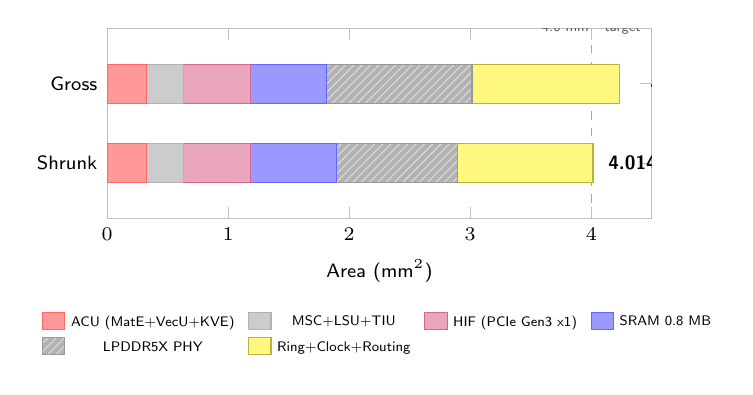
\begin{tikzpicture}
\begin{axis}[
  xbar stacked,
  bar width=14pt,
  width=8.5cm,
  height=4.0cm,
  xmin=0, xmax=4.5,
  ytick={1,2},
  yticklabels={Shrunk, Gross},
  yticklabel style={font=\sffamily\scriptsize},
  xlabel={Area (mm$^2$)},
  xlabel style={font=\sffamily\scriptsize},
  xticklabel style={font=\sffamily\scriptsize},
  legend style={
    font=\sffamily\tiny,
    at={(0.5,-0.45)}, anchor=north,
    legend columns=4, /tikz/every even column/.append style={column sep=3pt},
    draw=none, fill=none,
  },
  axis line style={gray!50},
  tick style={gray!50},
  enlarge y limits=0.7,
]
% Order: ACU, MSC+LSU+TIU, HIF, SRAM, PHY, ring+clock+routing
\addplot+[fill=red!40, draw=red!60] coordinates {(0.324,1) (0.324,2)};
\addplot+[fill=gray!40, draw=gray!60] coordinates {(0.31,1) (0.31,2)};
\addplot+[fill=purple!35, draw=purple!60] coordinates {(0.55,1) (0.55,2)};
\addplot+[fill=blue!40, draw=blue!60] coordinates {(0.71,1) (0.63,2)};
\addplot+[fill=gray!60, draw=gray!80, postaction={pattern=north east lines, pattern color=gray!30}] coordinates {(1.00,1) (1.20,2)};
\addplot+[fill=yellow!50, draw=yellow!70!black] coordinates {(1.12,1) (1.22,2)};
\legend{ACU (MatE+VecU+KVE), MSC+LSU+TIU, HIF (PCIe Gen3 x1), SRAM 0.8 MB, LPDDR5X PHY, Ring+Clock+Routing}
% 4.0 mm^2 target line (inside axis so axis cs: is valid)
\draw[dashed, gray!70, very thin] (axis cs:4,0.5) -- (axis cs:4,2.5);
\node[above, font=\sffamily\tiny, gray!70!black] at (axis cs:4,2.5) {4.0 mm$^2$ target};
\node[font=\sffamily\scriptsize, anchor=west, black] at (axis cs:4.06,1) {\bfseries 4.014};
\node[font=\sffamily\scriptsize, anchor=west, black] at (axis cs:4.41,2) {\bfseries 4.354};
\end{axis}
\end{tikzpicture}
\caption{Area accounting at PHY mid-case (\textit{Gross}, 4.354\,mm$^2$) and after the recommended shrink path---vendor PHY at 1.0\,mm$^2$ best case, I/O ring tightened to 80\,$\mu$m, activation buffer trimmed to 0.2\,MB---which lands at 4.014\,mm$^2$, within 0.4\% of the 4.0\,mm$^2$ target. Earlier spec drafts dropped the routing-overhead buffer (0.10\,mm$^2$) from the total and claimed 3.974\,mm$^2$; the pre-RTL audit corrected this.}
\label{fig:area}
\end{figure}

\subsection{Area and power budgets}

Table~\ref{tab:area} reports per-block area, verification surface, and risk classification; Figure~\ref{fig:area} visualizes the gross-versus-shrunk accounting. The gross total at the PHY mid-case (1.20\,mm$^2$) is 4.354\,mm$^2$, exceeding the 4\,mm$^2$ target by 0.354\,mm$^2$. The recommended shrink path---PHY landing at 1.0\,mm$^2$ vendor best case ($-0.20$\,mm$^2$), I/O ring tightened from 100\,$\mu$m to 80\,$\mu$m ($-0.06$\,mm$^2$), and the activation buffer shrunk from 0.3\,MB to 0.2\,MB ($-0.08$\,mm$^2$)---lands at 4.014\,mm$^2$, within 0.4\% of target. The shrink is contingent on the LPDDR5X x16 PHY vendor quote returning at or below 1.0\,mm$^2$; we discuss the LPDDR4X fallback in Section~\ref{sec:performance}.

Power decomposes to 2.6\,W typical decode and 3.3\,W peak prefill at 1\,GHz. The LPDDR5X PHY and DRAM together draw 0.72\,W (at the 7.5\,mW/Gbps planning figure for LPDDR5X-class memory and 96\,Gbps sustained). MatE at 50\% utilization is 0.32\,W (at the 5\,W/TOPS heuristic for INT8 systolic at 16\,nm), VecU 0.16\,W, SRAM 0.16\,W, the KVE holds a 0.05\,W placeholder (pending re-measurement for ChannelQuant), TIU 0.01\,W, MSC+LSU+HIF 0.50\,W. Whole-chip leakage at 16\,nm at 0.8\,V is approximately 0.70\,W. The M.2 2280 slot delivers approximately 10\,W per spec; we sit at 26\% of that envelope at typical decode.

% --- Table 1: Per-block area ---
\begin{table}[t]
\centering
\caption{Per-block area, verification surface, and risk class at PHY mid-case (1.20\,mm$^2$). $^\dagger$The KVE (ChannelQuant) block area at N16FFC is pending re-measurement; the gross total holds a 0.08\,mm$^2$ placeholder for it.}
\label{tab:area}
\setlength{\tabcolsep}{4pt}
\renewcommand{\arraystretch}{1.05}
\footnotesize
\begin{tabular}{lrrl}
\toprule
\textbf{Block} & \textbf{Area (mm$^2$)} & \textbf{Tests} & \textbf{Risk} \\
\midrule
MatE (8$\times$8 INT8$\times$INT4) & 0.10 & 50 & medium \\
VecU (8-lane SIMD)         & 0.144 & 25 & medium \\
KVE (ChannelQuant)         & TBD$^\dagger$ & 60 & low \\
MSC (LPDDR ctrl + xbar + BT) & 0.18 & 50 & medium \\
LSU (32-inst RISC)         & 0.10 & 30 & low \\
TIU (256\,B + accumulator) & 0.03 & 15 & low \\
HIF (PCIe Gen3 x1)         & 0.55 & 30 & medium \\
\midrule
SRAM (0.8\,MB, 4 banks)    & 0.71 & 20 & low \\
LPDDR5X x16 PHY (vendor)   & 1.20 & --- & high \\
\midrule
Clock + power grid         & 0.40 & --- & --- \\
Routing overhead           & 0.10 & --- & --- \\
I/O ring + pads + ESD      & 0.76 & --- & --- \\
\midrule
\textbf{Gross total}       & \textbf{4.354} & \textbf{280} & \\
With recommended shrinks   & 4.014 & --- & \\
\bottomrule
\end{tabular}
\end{table}

\subsection{Pre-RTL audit}

Before any HLS work begins we ran an explicit numerical audit of the spec and corrected eight inconsistencies. We document the audit here because each correction is a load-bearing decision that the rest of the chip integrates over.

\textit{KV bytes per token were 2.3$\times$ understated.} The bytes-per-token-per-layer formula in the original spec used $k_h \times d_h \times \mathrm{bpv}/8$, dropping the factor of 2 for K and V separately. We re-derived every capacity number against the correct $k_h \times d_h \times 2 \times \mathrm{bpv}/8$ formula. Under the ChannelQuant codec of record the bits-per-value is $\approx$4 (measured 4.13--4.38), and the per-model token capacities are pending re-derivation for the Qwen2-1.5B target.

\textit{The ``32K on-die'' claim was wrong.} With corrected math, no target model holds 32\,K context fully on-die per layer; the 0.4\,MB scratchpad holds on the order of $10^2$--$10^3$ tokens per layer depending on the KV-head layout. Long contexts serve via LPDDR5X streaming. The exact per-layout capacities and streaming overheads are pending re-derivation for ChannelQuant / Qwen2-1.5B.

\textit{MatE's INT16 accumulator was a real bug.} The original spec specified INT16 K-axis accumulators. INT8\,$\times$\,INT4 produces an 11-bit signed product; reducing $K{=}128$ requires 18 signed bits, saturating INT16 after approximately 64 accumulations in the worst case. Corrected to INT24 with an INT16 partial-product register inside each PE. The exact margin at the Qwen2-1.5B FFN dimensions is pending re-derivation.

\textit{The ``3--5$\times$ compute headroom'' claim was a derivation error.} In the bandwidth-bound regime, $\mathrm{GOPS}_{\mathrm{needed}} = 2 \cdot \mathrm{BW}_{\mathrm{GB/s}} / \mathrm{bytes}_{\mathrm{per\ param}}$, a constant across model sizes (because both numerator and denominator scale with bandwidth). The correct figure is a constant 1.6$\times$ headroom.

Additional corrections: the ``comfortable headroom at PHY = 1.0\,mm$^2$'' claim was misleading (the sensitivity sweep actually returns $+0.002$\,mm$^2$ at 1.0\,MB SRAM---exactly fits, no margin); the weight\_stream\_buffer was 0.05/0.15\,MB inconsistent (canonical 0.05); the total SRAM was 0.8/0.85/1.0\,MB inconsistent (canonical 0.8). The KV-codec bits-per-value figure that was reconciled at this audit has since been superseded by the ChannelQuant codec of record ($\approx$4 bits/value).

None of the corrections changed any architectural decision. Every fix was either a math error or a stale claim from an earlier iteration. We document them here because pre-RTL audits of this kind are, in our experience, frequently skipped in academic chip projects and frequently catch real bugs.

% =====================================================================
\section{Performance and the LPDDR PHY Tradeoff}
\label{sec:performance}
% =====================================================================

% --- Figure 3: Decode throughput vs model size ---
\begin{figure}[t]
\centering
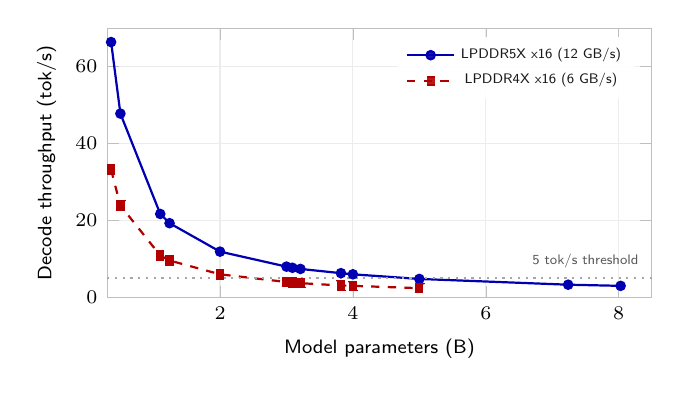
\begin{tikzpicture}
\begin{axis}[
  width=8.5cm, height=5.0cm,
  xlabel={Model parameters (B)},
  ylabel={Decode throughput (tok/s)},
  xlabel style={font=\sffamily\scriptsize},
  ylabel style={font=\sffamily\scriptsize},
  xticklabel style={font=\sffamily\scriptsize},
  yticklabel style={font=\sffamily\scriptsize},
  xmin=0.3, xmax=8.5, ymin=0, ymax=70,
  legend style={font=\sffamily\tiny, at={(0.97,0.97)}, anchor=north east, draw=none, fill=white, fill opacity=0.9},
  grid=both, grid style={gray!15},
  axis line style={gray!50},
  tick style={gray!50},
]
% LPDDR5X x16 (12 GB/s) -- bandwidth-bound: tok/s = BW / (params * bytes_per_param)
\addplot[mark=*, mark size=1.5pt, color=blue!70!black, thick] coordinates {
  (0.36, 66.4) (0.50, 47.8) (1.10, 21.7) (1.24, 19.3) (2.0, 11.9)
  (3.0, 8.0) (3.09, 7.7) (3.21, 7.4) (3.82, 6.3) (4.0, 6.0) (5.0, 4.8) (7.24, 3.3) (8.03, 3.0)
};
% LPDDR4X x16 (6 GB/s) - half BW
\addplot[mark=square*, mark size=1.5pt, color=red!70!black, thick, dashed] coordinates {
  (0.36, 33.2) (0.50, 23.9) (1.10, 10.9) (1.24, 9.6) (2.0, 6.0)
  (3.0, 4.0) (3.09, 3.9) (3.21, 3.7) (3.82, 3.1) (4.0, 3.0) (5.0, 2.4)
};
\addplot[domain=0.3:8.5, dotted, color=gray!70, thick] {5};
\node[font=\sffamily\tiny, anchor=south, color=gray!70!black] at (axis cs:7.5,5.2) {5 tok/s threshold};
\legend{LPDDR5X x16 (12 GB/s), LPDDR4X x16 (6 GB/s)}
\end{axis}
\end{tikzpicture}
\caption{Decode throughput versus model size under the two PHY options (a bandwidth-bound weight-streaming model, independent of the KV codec). Lambda's canonical target is up to 1.5\,B parameters (validated on Qwen2-1.5B), which sits comfortably above the 5\,tok/s threshold on the LPDDR5X x16 path with substantial headroom; the curve is drawn out to larger sizes to show where the bandwidth ceiling falls. The LPDDR4X fallback path caps lower (approximately 2.4\,B parameters above threshold). The larger data points ($\geq$3\,B) reflect the retired example set and are shown for context only.}
\label{fig:perf}
\end{figure}

Decode is bandwidth-bound at every reasonable model size. The largest model the chip can serve at a given throughput threshold derives directly from the bandwidth: $\mathrm{params}_{\max} = \mathrm{BW}_{\mathrm{GB/s}} \cdot t_{\mathrm{per\ tok}} / \mathrm{bytes}_{\mathrm{per\ param}}$. At LPDDR5X x16 (12\,GB/s sustained, $t=200$\,ms for 5\,tok/s, 0.5\,B/param for W4), the bandwidth ceiling is $\approx$4.8\,B parameters. The canonical target (up to 1.5\,B, validated on Qwen2-1.5B) sits well inside this ceiling, with substantial throughput headroom. Figure~\ref{fig:perf} shows the decode throughput curve across a range of model sizes; the larger points ($\geq$3\,B) reflect the retired example set and are shown for context only.

\subsection{The LPDDR5X-vs-LPDDR4X PHY tradeoff}

The dominant uncertainty in Lambda's area budget is the LPDDR5X x16 PHY footprint at 16\,nm, which is NDA-gated and which we estimate at 1.20\,mm$^2$ with $\pm 0.3$\,mm$^2$ real swing. The estimate is extrapolated from vendor x64 PHY data points; an authoritative number requires a written Synopsys or Cadence quote in Q2 2026. If the quote returns above 1.35\,mm$^2$, Lambda's recommended shrink path no longer closes at 4\,mm$^2$, and a fallback is required.

The natural fallback is LPDDR4X x16 with a Cadence PHY. LPDDR4X has been shipping at 16\,nm in multiple commercial parts since approximately 2018 and has public datasheets, in contrast to LPDDR5X's NDA-only 16\,nm references. The Cadence PHY for LPDDR4X at 16\,nm is approximately 1.0\,mm$^2$ with substantially less area variance ($\pm 0.15$\,mm$^2$). Adopting LPDDR4X frees approximately 0.2\,mm$^2$ of breathing room and materially de-risks the first-FinFET-PHY integration that is the chip's largest non-architectural risk.

The cost is bandwidth. LPDDR4X x16 sustains approximately 6\,GB/s, halving the bandwidth ceiling from approximately 4.8\,B parameters to approximately 2.4\,B at the 5\,tok/s threshold. The canonical target (Qwen2-1.5B and the $\leq$1.5\,B class---e.g.\ Llama-3.2-1B at 9.6\,tok/s, Qwen2.5-1.5B at 8.0\,tok/s) remains comfortably above threshold on either PHY, so the LPDDR4X fallback preserves the target class while trading away only the larger-model headroom. Adopting it keeps a fully public-datasheet PHY at materially lower tape-out risk.

The recommendation in our current planning is to commission both PHY quotes in parallel and gate the decision on the data. If the LPDDR5X x16 quote returns at or below 1.25\,mm$^2$ and a senior FinFET PD engineer is in place, the LPDDR5X path is correct; if the quote exceeds 1.35\,mm$^2$ or the PD-engineer prerequisite is not met, the LPDDR4X path is correct. Neither outcome kills the project.

\subsection{Comparison with prior art}

Table~\ref{tab:comp} positions Lambda against the closest reference points we are aware of. The mobile-NPU comparison is necessarily qualitative because the Apple Neural Engine~\cite{apple_foundation} and Qualcomm Hexagon NPU architectures are proprietary. Etched.ai's Sohu transformer ASIC~\cite{etched_sohu} sits at data-center scale on a substantially larger die. The academic-FPGA comparison reflects projects that target similar workloads at substantially larger die areas or older process nodes. Lambda's distinguishing positions are (i)~standalone operation at the small-model ($\leq$1.5\,B) class without a tightly-coupled SoC, (ii)~streaming per-channel KV compression (ChannelQuant) in silicon, (iii)~adaptive-precision KV via the TIU, and (iv)~open-source academic distribution.

% --- Table 2: Comparison (full page width to avoid clipping) ---
\begin{table*}[t]
\centering
\caption{Lambda versus the closest accelerator reference points.}
\label{tab:comp}
\setlength{\tabcolsep}{6pt}
\renewcommand{\arraystretch}{1.15}
\footnotesize
\begin{tabular}{lcccc}
\toprule
& \textbf{Lambda (this work)} & \textbf{Apple ANE}\textsuperscript{*} & \textbf{Qualcomm Hexagon NPU}\textsuperscript{*} & \textbf{Academic FPGA accelerators} \\
\midrule
Process                       & TSMC N16FFC          & $\le$N3                & $\le$N4                & 16/28\,nm                       \\
Die area                      & 4\,mm$^2$ (standalone) & integrated in SoC      & integrated in SoC      & 100+\,mm$^2$ (FPGA fabric)      \\
Model class @ 5\,tok/s        & $\le$1.5\,B params   & $\ge$3\,B              & $\ge$3\,B              & $\le$1\,B                       \\
KV compression                & ChannelQuant $\approx$4\,b/val & proprietary   & proprietary            & FP16 / INT8 (uniform)           \\
Adaptive-precision KV         & TIU (per-block)      & unknown                & unknown                & none                            \\
Per-channel INT4 KV codec     & yes (INT4$\cdot$FP16 dequant) & unknown       & unknown                & no                              \\
Open source                   & yes                  & no                     & no                     & varies                          \\
Form factor                   & M.2 2280 carrier     & integrated SoC         & integrated SoC         & dev board                       \\
Tape-out path                 & IMEC mini@sic 2.0    & internal               & internal               & FPGA bitstream (no tape-out)    \\
\bottomrule
\end{tabular}\\[2pt]
\raggedright\footnotesize\textsuperscript{*}\textit{Apple ANE and Qualcomm Hexagon NPU architectural details are proprietary; entries reflect publicly disclosed capabilities. Comparison is qualitative.}
\end{table*}

% =====================================================================
\section{Discussion}
\label{sec:discussion}
% =====================================================================

\subsection{What we deliberately excluded}

Lambda omits several mechanisms that are present in software-side frontier work. We document the exclusions because the omissions are deliberate and reversible in a future revision.

\textit{Multi-head Latent Attention (MLA).} DeepSeek-V2's MLA~\cite{mla} compresses Q/K/V into a low-rank latent space before the head split, reducing per-layer KV by approximately an order of magnitude versus standard MHA. Lambda's MSC and KVE both assume the conventional $k_h \times d_h$ KV layout. MLA would require a redesign of both blocks; we defer it for a future revision and document the gap explicitly.

\textit{Continuous batching and prefix sharing.} The single-session chip excludes multi-tenant serving primitives. We exclude them deliberately: a 4\,mm$^2$ die does not have area for the multi-session state, and the on-device deployment target does not benefit from them.

\textit{Mixture-of-Experts.} MoE routing requires a sparse-dispatch fabric that does not fit our area budget and that is not yet a dominant pattern in the small-model ($\leq$1.5\,B) class.

\textit{Mamba and other SSM blocks.} Selective state-space models~\cite{mamba} require different primitive operations from attention; the chip is not architected for them.

\textit{Multimodal vision/audio encoders.} Out of scope for the chip's text-only inference target.

\textit{Hardware speculative-decoding fabric.} Speculative decoding (Medusa~\cite{medusa}, EAGLE~\cite{eagle}) and multi-token prediction (DeepSeek-V3~\cite{deepseek_v3}) are architecturally compatible: the host coordinates draft tokens, and the chip runs the verifier pass through a standard batched-$N$ decode schedule. We do not include a dedicated speculative-decoding accelerator on-die; the LSU schedule is general enough to accommodate the pattern.

\subsection{IP clearance: the Etched patent}

Etched.ai's US patent 2024/0419516\,A1~\cite{etched_patent} describes an AI hardware platform comprising two structurally separated circuits on a single IC: a systolic array for operations that do not consume past-token data and a self-attention circuit for operations that do. Lambda's MatE is a \textit{single} 8$\times$8 systolic that mode-multiplexes between weight-stationary (for the no-past-token-data operations the patent describes as belonging to its systolic array) and output-stationary (for the past-token-data operations the patent describes as belonging to its self-attention circuit). The structural separation that grounds the patent's claim is absent in Lambda's design; the mode-switch is a CSR bit, not two circuits.

Our reading is that Lambda is outside the claim scope, but a defensive review with our institutional technology transfer office is the appropriate next step before silicon commit. The patent does highlight a real scheduling distinction we adopt explicitly: the LSU schedule treats weight-matmul tiles and attention-matmul tiles as separate dispatch primitives with separate optimization targets (K-axis size, operand stationarity).

\subsection{Risks and open questions}

The largest non-architectural risk is the LPDDR5X x16 PHY integration: this is the team's first FinFET-era PHY tape-out, and the 1.20\,mm$^2$ estimate has $\pm 0.3$\,mm$^2$ real swing. Mitigation is the vendor quote (Q2 2026) and a senior FinFET physical-design engineer in place by Q3 2026; the LPDDR4X fallback (Section~\ref{sec:performance}) is the documented release valve.

The IMEC mini@sic 2.0 actual pricing for 4\,mm$^2$ N16FFC is non-public; the \$60--100\,K range is an academic-discount-tier estimate. A direct quote via \texttt{eptsmc@imec.be} is the first concrete action item on the project's gantt.

% =====================================================================
\section{Conclusion}
% =====================================================================

We have presented Lambda, a 4\,mm$^2$ open-source academic transformer-decode ASIC at TSMC N16FFC that serves the small-model ($\leq$1.5\,B, validated on Qwen2-1.5B) on-device deployment regime at 6--8\,tok/s in 2.6\,W. The chip integrates a streaming silicon implementation of \emph{ChannelQuant}---per-channel INT4 keys, per-token INT4 values, and a static top-$k$ FP16 outlier-channel lane, following the KIVI~\cite{kivi} / KVQuant~\cite{kvquant} recipe---together with the first silicon implementation of adaptive-precision KV cache management via on-die attention-entropy accumulation (the TIU), in an open-source academic standalone accelerator. We have documented the design-space exploration, the LPDDR5X-versus-LPDDR4X PHY tradeoff, and an explicit pre-RTL audit. The KV-compression block's physical PPA at N16FFC (area, power, $F_\mathrm{max}$), and the target-model throughput and capacity figures, are pending re-measurement and re-derivation for ChannelQuant on Qwen2-1.5B. The next phase is high-level synthesis of the MatE processing element and the KVE ChannelQuant datapath---the two long poles. The full architecture specification, the audit log, the literature review, and the per-block HLS scaffolding are publicly available at \texttt{github.com/LonghornSilicon/architecture}.

\section*{Acknowledgments}

The author thanks the UT Austin Computer Architecture Lab, the IMEC / Europractice mini@sic 2.0 program, and the broader open-source quantization research community whose work this chip integrates.

% =====================================================================
\bibliographystyle{IEEEtran}
\bibliography{lambda}

\end{document}
